\trilingualchapter{Supply Chain Management: The Backbone of Quality}{供应链管理:质量的支柱}{Lieferkettenmanagement: Das Rückgrat der Qualität}{}

A restaurant's success depends not only on great food and service but also on a reliable, efficient supply chain. This chapter explores how Sue and Owen built relationships with suppliers, managed inventory, and ensured consistent quality while controlling costs.

\section{Understanding the Restaurant Supply Chain | 理解餐厅供应链 | Das Restaurant-Lieferkettennetzwerk verstehen}

The restaurant supply chain encompasses all activities from sourcing raw materials to delivering finished dishes to customers. Sue and Owen recognized that an effective supply chain is invisible to customers but essential to operations.

\subsection{Supply Chain Components | 供应链组成部分 | Lieferkettenkomponenten}

\begin{enumerate}
    \item \textbf{Suppliers}: Farmers, distributors, specialty vendors
    \item \textbf{Purchasing}: Ordering, negotiation, relationship management
    \item \textbf{Receiving}: Inspection, quality control, documentation
    \item \textbf{Storage}: Proper handling, rotation, inventory management
    \item \textbf{Production}: Kitchen operations using supplies
    \item \textbf{Distribution}: Getting food to customers
\end{enumerate}

\begin{figure}[h]
\centering
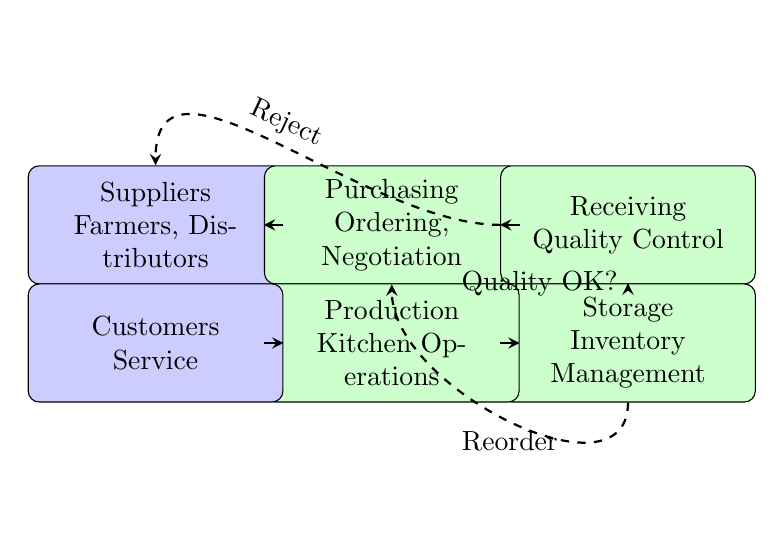
\begin{tikzpicture}[
    node distance=2cm,
    auto,
    block/.style={rectangle, draw, fill=blue!20, text width=3cm, text centered, rounded corners, minimum height=1.5cm},
    process/.style={rectangle, draw, fill=green!20, text width=3cm, text centered, rounded corners, minimum height=1.5cm},
    decision/.style={diamond, draw, fill=yellow!20, text width=2.5cm, text centered, aspect=2},
    arrow/.style={thick,->,>=stealth}
]
    % Nodes
    \node [block] (suppliers) {Suppliers\\Farmers, Distributors};
    \node [process, right of=suppliers, xshift=1cm] (purchasing) {Purchasing\\Ordering, Negotiation};
    \node [process, right of=purchasing, xshift=1cm] (receiving) {Receiving\\Quality Control};
    \node [process, below of=receiving, yshift=0.5cm] (storage) {Storage\\Inventory Management};
    \node [process, left of=storage, xshift=-1cm] (production) {Production\\Kitchen Operations};
    \node [block, left of=production, xshift=-1cm] (customers) {Customers\\Service};
    
    % Arrows
    \draw [arrow] (suppliers) -- (purchasing);
    \draw [arrow] (purchasing) -- (receiving);
    \draw [arrow] (receiving) -- node {Quality OK?} (storage);
    \draw [arrow] (storage) -- (production);
    \draw [arrow] (production) -- (customers);
    
    % Feedback loop
    \draw [arrow, dashed] (receiving) to[out=180, in=90] node [above, sloped] {Reject} (suppliers);
    \draw [arrow, dashed] (storage) to[out=270, in=270] node [below] {Reorder} (purchasing);
\end{tikzpicture}
\caption{Restaurant Supply Chain Flow}
\label{fig:supply_chain_flow}
\end{figure}

\section{Building Supplier Relationships | 建立供应商关系 | Lieferantenbeziehungen aufbauen}

Sue and Owen understood that strong supplier relationships are partnerships, not just transactions. They invested time in finding and developing relationships with the right suppliers.

\subsection{Identifying Suppliers | 识别供应商 | Lieferanten identifizieren}

\subsubsection{Primary Categories}
\begin{itemize}
    \item \textbf{Broadline distributors}: One-stop shops (Sysco, US Foods, etc.)
    \item \textbf{Specialty vendors}: Specific products (artisan bread, local produce)
    \item \textbf{Local farmers}: Fresh produce, meats, dairy
    \item \textbf{Beverage distributors}: Wine, beer, spirits, non-alcoholic
    \item \textbf{Equipment and supplies}: Smallwares, cleaning supplies, disposables
\end{itemize}

\subsubsection{Selection Criteria}
\begin{itemize}
    \item Product quality and consistency
    \item Reliability and delivery schedules
    \item Pricing and payment terms
    \item Minimum order requirements
    \item Geographic proximity
    \item Customer service and support
    \item Sustainability practices
    \item Certifications (organic, fair trade, etc.)
\end{itemize}

\subsection{Supplier Evaluation Process | 供应商评估流程 | Lieferantenbewertungsprozess}

Sue and Owen created a systematic approach to evaluating suppliers:

\begin{table}[h]
\centering
\begin{tabular}{lcc}
\toprule
\textbf{Criteria} & \textbf{Weight} & \textbf{Score (1-10)} \\
\midrule
Product quality & 25\% & \\
Reliability & 20\% & \\
Pricing & 15\% & \\
Service level & 15\% & \\
Sustainability & 10\% & \\
Payment terms & 10\% & \\
Geographic proximity & 5\% & \\
\midrule
\textbf{Total} & \textbf{100\%} & \\
\bottomrule
\end{tabular}
\caption{Supplier Evaluation Matrix}
\end{table}

\subsection{Developing Partnerships | 发展合作伙伴关系 | Partnerschaften entwickeln}

Once suppliers were selected, Sue and Owen focused on building partnerships:

\begin{itemize}
    \item \textbf{Regular communication}: Weekly check-ins, quarterly reviews
    \item \textbf{Forecasting}: Sharing sales projections and menu changes
    \item \textbf{Feedback}: Providing honest feedback on quality and service
    \item \textbf{Fair treatment}: Paying invoices on time, respecting contracts
    \item \textbf{Collaboration}: Working together on menu development and specials
    \item \textbf{Exclusivity agreements}: When appropriate, for mutual benefit
\end{itemize}

\section{Purchasing Strategy | 采购策略 | Einkaufsstrategie}

\subsection{Purchasing Methods | 采购方法 | Einkaufsmethoden}

\subsubsection{Direct Purchasing}
\begin{itemize}
    \item Buying directly from producers (farmers, fishermen)
    \item Often better quality and pricing
    \item Requires more coordination and logistics
    \item Best for specialty items and local sourcing
\end{itemize}

\subsubsection{Distributor Purchasing}
\begin{itemize}
    \item Using broadline or specialty distributors
    \item Convenience and consolidated deliveries
    \item May have higher costs but lower logistics burden
    \item Best for high-volume, standard items
\end{itemize}

\subsubsection{Hybrid Approach}
Sue and Owen used a hybrid approach:
\begin{itemize}
    \item Broadline distributor for staples (flour, oils, cleaning supplies)
    \item Specialty vendors for unique items (artisan cheeses, specialty meats)
    \item Local farmers for seasonal produce
    \item Direct relationships for signature ingredients
\end{itemize}

\subsection{Purchasing Procedures | 采购程序 | Einkaufsverfahren}

\subsubsection{Ordering Process}
\begin{enumerate}
    \item Inventory assessment (daily or weekly)
    \item Menu requirements review
    \item Order creation (using POS or inventory system)
    \item Approval and submission
    \item Confirmation and delivery scheduling
    \item Receiving and inspection
\end{enumerate}

\subsubsection{Order Frequency}
\begin{itemize}
    \item \textbf{Daily}: Highly perishable items (fresh produce, seafood)
    \item \textbf{2-3 times per week}: Perishable items (dairy, meats)
    \item \textbf{Weekly}: Semi-perishable items (bread, some produce)
    \item \textbf{Bi-weekly or monthly}: Dry goods, frozen items, supplies
\end{itemize}

\subsection{Cost Management | 成本管理 | Kostenmanagement}

\subsubsection{Pricing Strategies}
\begin{itemize}
    \item \textbf{Volume discounts}: Negotiate better prices for larger orders
    \item \textbf{Contract pricing}: Lock in prices for stability
    \item \textbf{Market pricing}: Accept market fluctuations for flexibility
    \item \textbf{Competitive bidding}: Regular comparison shopping
\end{itemize}

\subsubsection{Cost Control Measures}
\begin{itemize}
    \item Set target food cost percentages (typically 28-35\%)
    \item Regular price comparisons
    \item Menu engineering to optimize profitability
    \item Waste reduction programs
    \item Inventory turnover optimization
\end{itemize}

\section{Receiving and Quality Control | 收货与质量控制 | Wareneingang und Qualitätskontrolle}

\subsection{Receiving Procedures | 收货程序 | Wareneingangsverfahren}

Sue and Owen established strict receiving procedures:

\subsubsection{Receiving Checklist}
\begin{itemize}
    \item Verify order accuracy (quantities, items)
    \item Check delivery temperature (especially for perishables)
    \item Inspect quality (freshness, appearance, packaging)
    \item Verify pricing matches purchase order
    \item Check expiration dates
    \item Document any issues (damages, shortages, quality problems)
    \item Sign delivery receipt only after inspection
    \item Immediately move items to proper storage
\end{itemize}

\subsubsection{Quality Standards}

They established quality standards for each category:

\begin{itemize}
    \item \textbf{Produce}: Fresh, no bruising or wilting, proper ripeness
    \item \textbf{Meat}: Proper color, no off odors, correct temperature
    \item \textbf{Seafood}: Clear eyes, firm flesh, ocean smell (not fishy)
    \item \textbf{Dairy}: Proper temperature, no expired dates
    \item \textbf{Dry goods}: Intact packaging, no pests, proper storage
\end{itemize}

\subsection{Rejection Procedures | 拒收程序 | Ablehnungsverfahren}

When items don't meet standards:
\begin{enumerate}
    \item Document the issue (photos if possible)
    \item Contact supplier immediately
    \item Reject items (don't accept and negotiate later)
    \item Request replacement or credit
    \item Update inventory records
    \item Follow up to prevent recurrence
\end{enumerate}

\section{Inventory Management | 库存管理 | Bestandsverwaltung}

\subsection{Inventory Systems | 库存系统 | Bestandssysteme}

\subsubsection{Perpetual Inventory}
\begin{itemize}
    \item Continuous tracking using POS or inventory software
    \item Real-time visibility into stock levels
    \item Automatic reorder points
    \item More accurate but requires discipline
\end{itemize}

\subsubsection{Periodic Inventory}
\begin{itemize}
    \item Physical counts at regular intervals (weekly, monthly)
    \item Calculate usage between counts
    \item Simpler but less precise
    \item Good for smaller operations
\end{itemize}

\subsubsection{Hybrid Approach}
Sue and Owen used a hybrid:
\begin{itemize}
    \item Perpetual system for high-value items (meat, seafood, alcohol)
    \item Periodic counts for lower-value items (dry goods, supplies)
    \item Weekly full inventory for accuracy
\end{itemize}

\subsection{Storage and Organization | 存储与组织 | Lagerung und Organisation}

\subsubsection{Storage Principles}
\begin{itemize}
    \item \textbf{FIFO (First In, First Out)}: Always use oldest items first
    \item \textbf{Proper labeling}: Date received, expiration date, contents
    \item \textbf{Organization}: Logical grouping, easy access
    \item \textbf{Temperature control}: Maintain proper storage temperatures
    \item \textbf{Security}: Control access, prevent theft
\end{itemize}

\subsubsection{Storage Areas}
\begin{itemize}
    \item \textbf{Dry storage}: Cool, dry, well-ventilated, organized shelves
    \item \textbf{Refrigerated}: 32-40°F, organized by category
    \item \textbf{Frozen}: 0°F or below, proper packaging
    \item \textbf{Chemical storage}: Separate, locked, away from food
\end{itemize}

\subsection{Inventory Control | 库存控制 | Bestandskontrolle}

\subsubsection{Key Metrics}
\begin{itemize}
    \item \textbf{Food cost percentage}: (Cost of goods sold / Sales) × 100
    \item \textbf{Inventory turnover}: Cost of goods sold / Average inventory
    \item \textbf{Theft and waste}: Track shrinkage
    \item \textbf{Par levels}: Minimum stock levels for reordering
\end{itemize}

\subsubsection{Waste Reduction}
\begin{itemize}
    \item Menu planning to use all parts of ingredients
    \item Proper portion control
    \item Creative use of leftovers (staff meals, specials)
    \item Composting programs
    \item Regular inventory to prevent over-ordering
\end{itemize}

\section{Supply Chain Technology | 供应链技术 | Lieferkettentechnologie}

\subsection{Inventory Management Software | 库存管理软件 | Bestandsverwaltungssoftware}

Modern restaurants use technology to manage supply chains:

\begin{itemize}
    \item \textbf{POS integration}: Automatic inventory deduction from sales
    \item \textbf{Ordering systems}: Streamlined ordering processes
    \item \textbf{Receiving apps}: Mobile receiving and inspection
    \item \textbf{Analytics}: Cost tracking, usage patterns, forecasting
\end{itemize}

\subsection{Benefits of Technology | 技术的好处 | Vorteile der Technologie}

\begin{itemize}
    \item Reduced manual errors
    \item Time savings
    \item Better data for decision-making
    \item Improved accuracy
    \item Cost visibility
\end{itemize}

\section{Sustainability in the Supply Chain | 供应链中的可持续性 | Nachhaltigkeit in der Lieferkette}

Sue and Owen prioritized sustainability:

\subsection{Sustainable Practices | 可持续实践 | Nachhaltige Praktiken}
\begin{itemize}
    \item \textbf{Local sourcing}: Reduce transportation, support community
    \item \textbf{Seasonal menus}: Work with natural cycles
    \item \textbf{Organic and sustainable}: When possible and affordable
    \item \textbf{Packaging reduction}: Minimize waste
    \item \textbf{Supplier partnerships}: Work with like-minded suppliers
\end{itemize}

\subsection{Benefits | 好处 | Vorteile}
\begin{itemize}
    \item Environmental responsibility
    \item Community support
    \item Marketing advantage
    \item Often better quality
    \item Customer appeal
\end{itemize}

\section{Managing Supply Chain Challenges | 管理供应链挑战 | Lieferkettenherausforderungen bewältigen}

\subsection{Common Challenges | 常见挑战 | Häufige Herausforderungen}

\begin{itemize}
    \item \textbf{Price volatility}: Market fluctuations
    \item \textbf{Quality inconsistency}: Supplier variations
    \item \textbf{Delivery issues}: Late or incomplete deliveries
    \item \textbf{Seasonal availability}: Product availability changes
    \item \textbf{Storage limitations}: Space constraints
    \item \textbf{Cash flow}: Payment timing
\end{itemize}

\subsection{Solutions | 解决方案 | Lösungen}

\begin{itemize}
    \item Maintain backup suppliers
    \item Build inventory buffers for critical items
    \item Flexible menu that adapts to availability
    \item Strong relationships for priority service
    \item Clear contracts and expectations
    \item Regular communication and problem-solving
\end{itemize}

\trilingualsection{Key Takeaways}{关键要点}{Wichtige Erkenntnisse}{}

\begin{itemize}
    \item Supply chain is foundational to restaurant success
    \item Strong supplier relationships are partnerships
    \item Quality control at receiving prevents problems
    \item Effective inventory management controls costs
    \item Technology improves accuracy and efficiency
    \item Sustainability can be a competitive advantage
    \item Flexibility and backup plans are essential
\end{itemize}

With a solid supply chain in place, Sue and Owen could focus on the heart of their restaurant: creating exceptional food and delivering outstanding service. The next chapter explores food service operations in detail.
